%!TEX root = lections.tex
Рассмотрим узкий бассейн с жидкостью (должен быть достаточно длинным):
\begin{figure}[H]
	\centering
	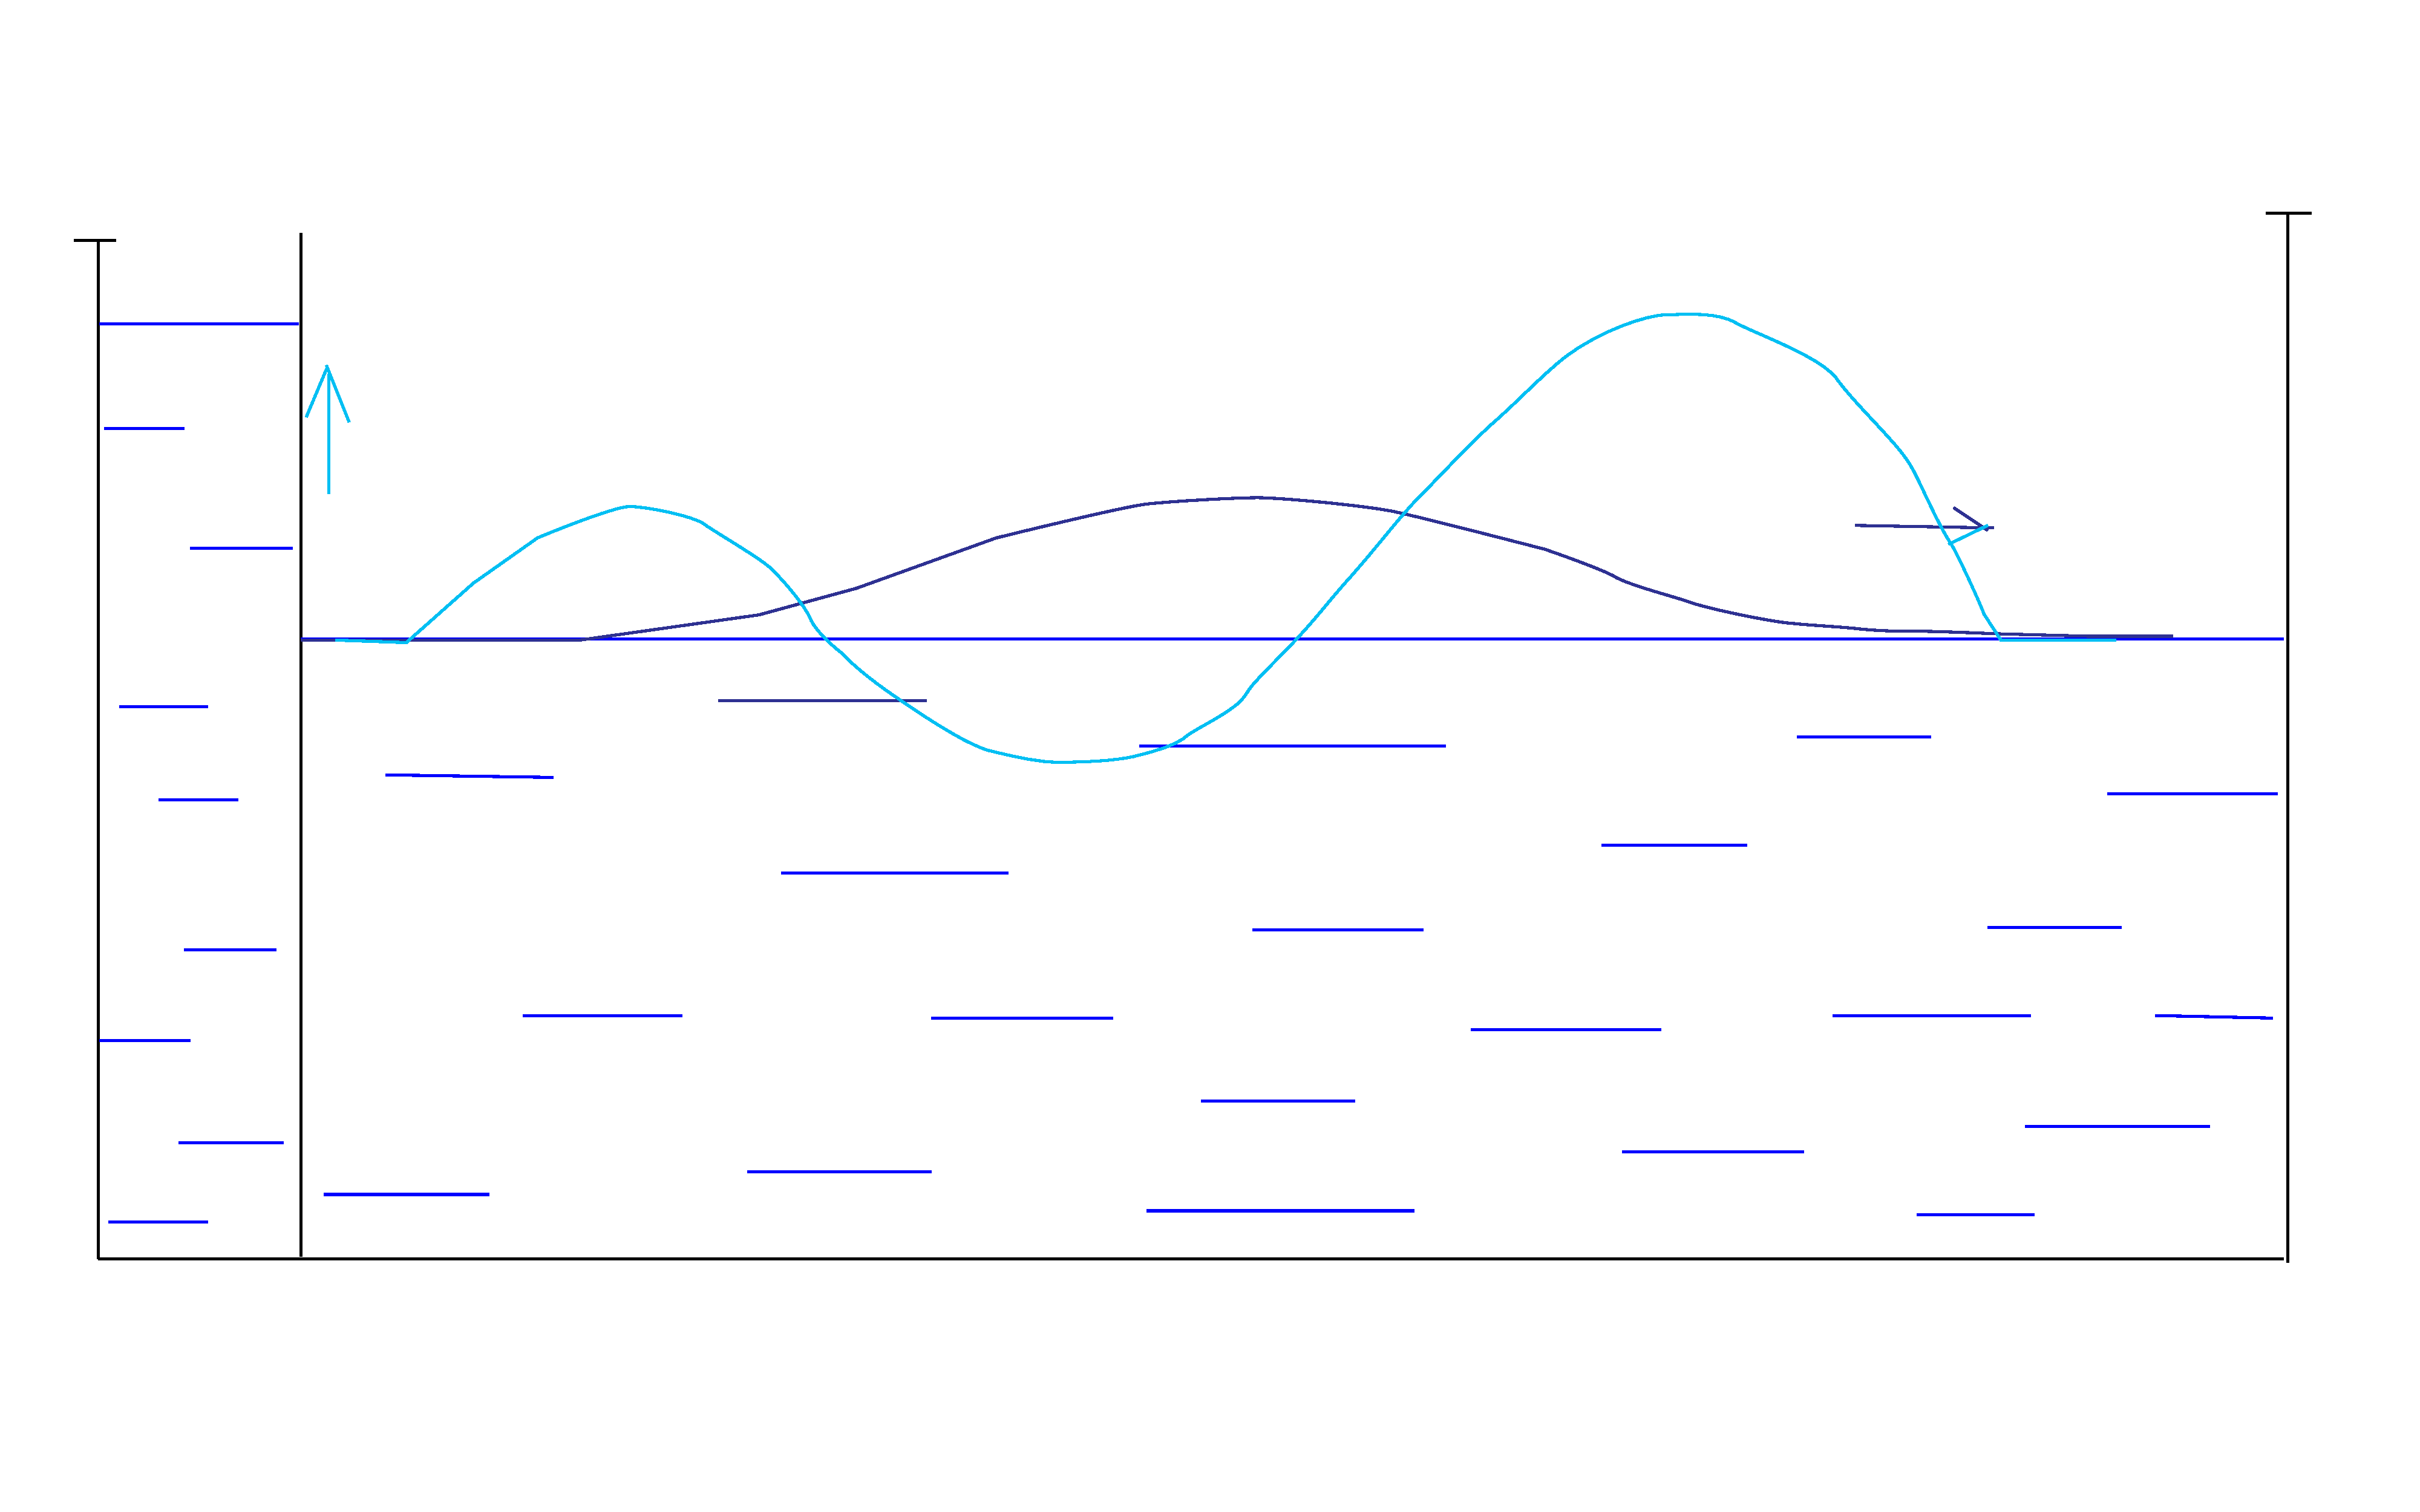
\includegraphics[width=0.4\linewidth]{fig/fig18.pdf}   
\end{figure}

Подбирают соотношение масс воды в емкостях. Резко поднимают задвижку. В зависимости от соотношения масс воды, могут побежать разные волны, разное количество холмов. 

Канал, который мы рассматриваем, мелкий, средней глубины $l$; $l+\eta(x,t)$. Поверим на слово: 
\begin{equation*}
	\pdv{\eta}{t}=\frac32 \sqrt{\frac{g}{l}}\pdv{}{x}\qty(\frac32 \alpha \eta+\frac12 \eta^2+\frac13 \sigma \pdv[2]{\eta}{x}),
\end{equation*}
где $\sigma=\frac{l^3}{3}-\frac{Tl}{\rho g}$, $\alpha$-произвольная константа, $T$ - коэффициент поверхностного натяжения, $\rho$ - плотность жидкости.

Преобразовав, получим
\begin{equation}
	\pdv{U}{t}+U\pdv{U}{x}+\beta \pdv[3]{U}{x}=0.
	\label{eq:33}
\end{equation}
$\beta$ - некоторая константа, а последнее слагаемое характеризует дисперсию. Видно, что уравнение простой волны дополняется дисперсией. (К экзамену построить дисперсионную характеристику). 

Пусть есть квадратичная среда, в нее запускают волну $e^{i(\omega_o t+kx)}$. Среда нелинейная и без дисперсии. При таких условиях квадратичная среда порождает новые частоты. $\omega_o$ порождает $2\omega_o$. Если нет дисперсии, то нет пространственных масштабов. $2\omega_o$ порождает $3\omega_o$ и так далее, лавинно. Спектр стремится в бесконечность. 
\begin{figure}[H]
	\centering
	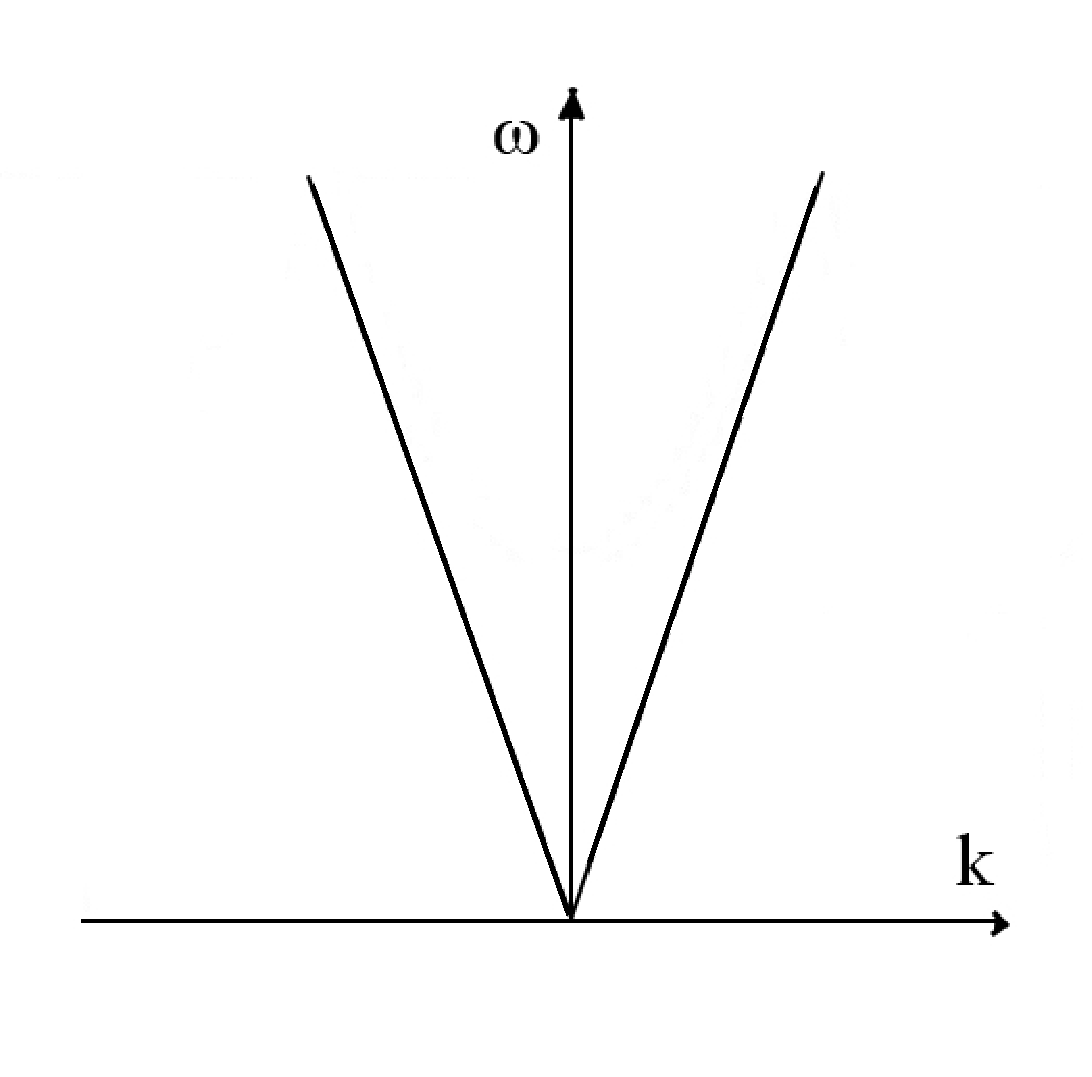
\includegraphics[width=0.4\linewidth]{fig/fig4.pdf}   
\end{figure}

Теперь включим дисперсию (в данном случае - высокочастотную). Она ограничивает частотный рост и стабилизирует волну. 

Будем искать решение уравнения \eqref{eq:33} в виде $U=U(x-Vt)$:
\begin{equation}
	-\pdv{U}{\xi}+U\pdv{U}{\xi}+\beta \pdv[3]{U}{\xi}=0.
	\label{eq:34}
\end{equation}

Интегрируя:
\begin{equation}
	\beta \pdv[2]{U}{\xi}+\frac{U^2}{2}-VU=0.
	\label{eq:35}
\end{equation}

Это есть уравнение нелинейного осциллятора. Для простоты константу интегрирования приравняли  к нулю, что дает уровень, откуда изменяется $U(x,t)$.
\begin{equation}
	\begin{cases}
		\dot{U}=y \\
		\beta \dot{y} =VU-\frac{U^2}{2}.		
	\end{cases}
	\label{eq:36}
\end{equation}

Получили систему для нелинейного осциллятора.
\begin{gather*}
	\beta \frac{y^2}{2}+E_{\text{п}} = const, \\ E_{\text{п}} = \frac{U^3}{6}-V\frac{U^2}{2}
\end{gather*}
\begin{figure}[H]
	\centering
	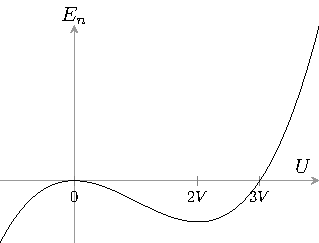
\includegraphics[width=0.4\linewidth]{fig/fig19.pdf}   
\end{figure}

Фазовый портрет:
\begin{figure}[H]
	\centering
	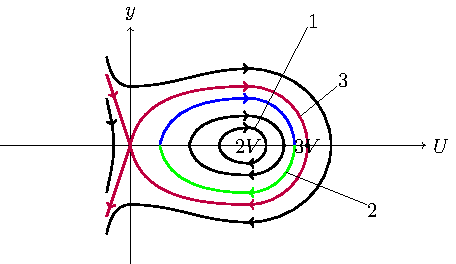
\includegraphics[width=0.5\linewidth]{fig/fig20.pdf}   
\end{figure}
Солитоном и является эта, покрашенная в восхитительный purple, гомоклиническая орбита.

22.04

Напомню, что дифференцирование в системе \eqref{eq:36} производится по бегущей координате. 

Вернемся к фазовому портрету. Неограниченные траектории лишены физического смысла, поэтому нас интересуют только ограниченные, то есть те, что находятся внутри петли сепаратрис, включая ее саму.

Пусть 1 - траектория вблизи состояния равновесия центр. Она замкнутая, колебание близко к гармоническому. Колебание происходит на фоне колебаний 2V. Таких колебаний континуум. 
\begin{figure}[H]
	\centering
	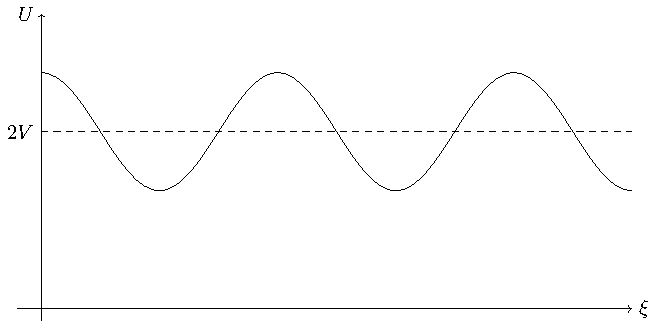
\includegraphics[width=0.4\linewidth]{fig/fig21.pdf}   
\end{figure}

Выберем 2 - вблизи седла, но все еще внутри гомоклинической орбиты. Выберем точку и положим при $\xi=0$ амплитуда максимальна. При движении по траектории к седлу (зеленым), U убывает. 
\begin{figure}[H]
	\centering
	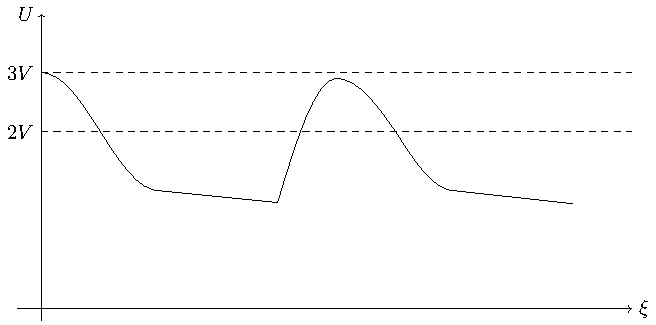
\includegraphics[width=0.4\linewidth]{fig/fig22.pdf}   
\end{figure}
Около самого состояния равновесия скорость мала, движение в ее окрестности будет проходить медленно. В конце концов, при выходе из окрестности состояния равновесия, скорость опять увеличится. Мы получим профиль, так называемой, кноидальной волны, которая далека от гармонической. Волны такие, потому что система нелинейная. 
Если брать траектории все ближе к седлу, полка будет увеличиваться. В конце концов, когда попадем на петлю:

Для того, чтобы нарисовать профиль в область $\xi<0$, нужно пройти по траектории в обратную сторону (синим). Рисунок качественный, нарисован из понимания поведения функции на концах и зная максимальную амплитуду. 
\begin{figure}[H]
	\centering
	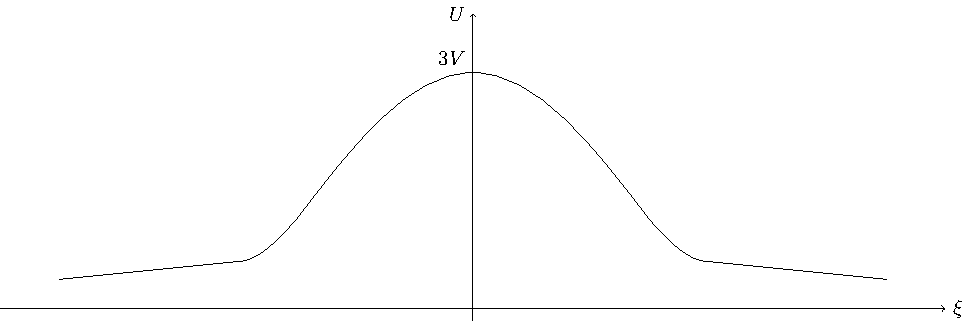
\includegraphics[width=0.4\linewidth]{fig/fig23.pdf}   
\end{figure}
Получившийся одиночный холм - это математический образ солитона. Точка 0 - решение, там нет пересечения траекторий, они стремятся туда асимптотически. 

Запишем наше уравнение в виде:

\begin{equation}
	\beta\dv[2]{U}{\xi}=VU-\frac{U^2}{2}
	\label{eq:37}
\end{equation}

Решение будем искать в виде:
\begin{equation}
	U=\frac{U_{max}}{\ch^2{(\xi / \Delta)}}
	\label{eq:38}
\end{equation}

Введенные параметры: $U_{max}, \Delta, V$ (V скрыто в $\xi=x-Vt$).
\begin{equation}
	\dv[2]{U}{\xi}=-2\frac{U_m}{\Delta^2}\frac{(3-2\ch^2{\xi / \Delta)}}{\ch^4{(\xi / \Delta)}}
	\label{eq:39}
\end{equation}
\begin{gather*}
	\frac{2\beta U_m}{\Delta^2}\frac{(3-2\ch^2{(\xi / \Delta))}}{\ch^4{(\xi / \Delta)}}=\frac{U_m V}{\ch^2{(\xi / \Delta)}}-\frac{U_m^2}{2\ch^4{(\xi / \Delta)}}.
\end{gather*}

Знаменатель не обращается в ноль.
\begin{gather*}
	-2\beta[3-2\ch^2{(\xi / \Delta)}]=\Delta^2 \ch^2{(\xi / \Delta)}V-\frac{U_m \Delta^2}{2}, \\
	-6\beta=\frac{U_m \Delta^2}{2}, \\
	4\beta=\Delta^2V.
\end{gather*}
\begin{equation}
	U_m \Delta^2= 12\beta,
	\label{eq:40}
\end{equation}
\begin{equation}
	\Delta^2V=4\beta.
	\label{eq:41}
\end{equation}
Параметры связаны, но их 3, а условия 2. Задав один, два других найдутся из \eqref{eq:40} и \eqref{eq:41}. $\beta$ характеризует дисперсию, не относится к самому солитону. V - скорость солитона, $U_m$ - его высота, $\Delta$ оказывается шириной. Ширина солитона вычисляется на уровне $U=\frac{4U_m}{2+e}$. 

Из уравнения \eqref{eq:41} следует, что, чем шире солитон, тем меньше его скорость: $V=\frac{4\beta}{\Delta^2}$. Из \eqref{eq:40}, что тогда и меньше амплитуда: $U_m=\frac{12\beta}{\Delta^2}$.

Если в диссипативной системе есть петля, то при изменении параметров она разрушается.Есть всего одна траектория, формирующая солитон. Солитоны устойчивы относительно большого числа начальных распределений. 

\subsubsection{Устойчивость солитона}
Замечание: рассмотрим уравнение Шредингера для определения статистического состояния. 
\begin{equation}
	\dv[2]{\psi}{x}+[U(x)+\epsilon]\psi=0.
	\label{eq:42}
\end{equation}

$U(x)>0, ~U\rightarrow 0$ при $x\rightarrow \pm \infty$

Есть решение, когда спектр дискретный: $\epsilon=\epsilon_n, \psi, \psi' \rightarrow 0$ при $x\rightarrow \pm \infty$.\

Существует связь между \eqref{eq:41} и устойчивостью солитонов уравнения Кортевега - де Фриза. Надо подставить нормированное решение:
\begin{equation*}
	\dv[2]{\psi}{x}+[\frac{1}{6\beta}U(x,t)+\epsilon]\psi=0.
\end{equation*}

Покажем, что, если речь о солитоне, то $\epsilon$ не будет зависеть от t.
\begin{equation*}
	U(x,t)=-6\beta(\frac{\psi''}{\psi}+\epsilon),
\end{equation*}
здесь $'$ - дифференцирование по x. Подставим в уравнение Кортевега - де Фриза:
\begin{equation*}
	\pdv{U}{t}+U\pdv{U}{x}+\beta \pdv[3]{U}{x}=0.
\end{equation*}
\begin{equation}
	\psi^2\dv{\epsilon}{t}=(\psi'A-A\psi').
	\label{eq:43}
\end{equation}
\begin{equation*}
	A(x,t)=6\beta(\frac1{\beta}\pdv{\psi}{t}-3\frac{\psi'\psi''}{\psi}+\psi'''-\frac{\epsilon}{6}\psi').
\end{equation*}

Проинтегрируем \eqref{eq:42} по переменной x в бесконечных пределах. Вспомним, что $\psi, \psi' \rightarrow 0$ при $x\rightarrow \pm \infty$. Получим:
\begin{equation*}
	\dv{\epsilon}{t}\int^{+\infty}_{-\infty}\psi^2dx=0.
\end{equation*}

В силу нормировки интеграл не равен нулю. Следовательно, $\dv{\epsilon}{t}=0$ и $\epsilon\neq \epsilon(t)$.
\begin{equation*}
	U(x,t)=U_{max}c\ch^{-2}(\frac{x-Vt}{\Delta}).
\end{equation*}

Здесь t можно выбрать любое. Положим, $t=0$.
\begin{equation}
	\psi''+(U_0 \ch^{-2}\alpha x+\epsilon)\psi=0.
	\label{eq:44}
\end{equation}
\begin{equation*}
	U_0=\frac{U_m}{6\beta},~\alpha=\frac1{\Delta}.
\end{equation*}

Пользуясь случаем, передаем приветы и спасибо третьему тому Ландау-Лившица, параграф 23, задача 4, где это уравнение решено. Спектр:
\begin{gather*}
	\epsilon_n=-\alpha(s-n), n=0,1,2,\dots;~n<s \\ s=\frac12(-1+\sqrt{1+\frac{4U_0}{\alpha^2}})=\frac12(-1+\sqrt{\frac{4U_m\Delta^2}{6\beta}})=\frac12(-1+3)=1 \\ \epsilon_n=-\alpha(1-n) \\ n=0:~ \epsilon_0=-\alpha^2=-\frac{4U_m}{12\beta}.
\end{gather*}

Если в уравнение Шредингера подставить уравнение солитона, такому потенциалу соответствует одно собственное значение. Пусть в начальный момент есть распределение (положительно определенное, но не совпадающее с солитоном). Подставляя его в уравнения Шредингера, решив, получим столько $\epsilon_j$, сколько солитонов может существовать при таких начальных условиях.
\begin{figure}[H]
	\centering
	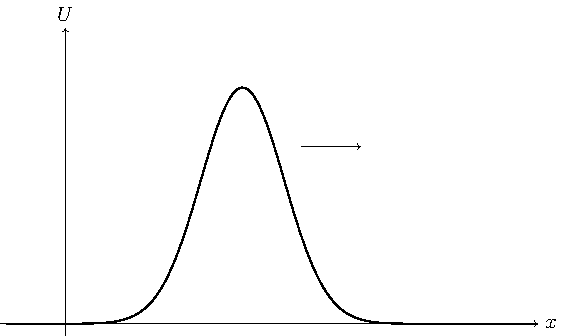
\includegraphics[width=0.4\linewidth]{fig/fig25.pdf}   
\end{figure}

Пусть $j=3$:
\begin{figure}[H]
	\centering
	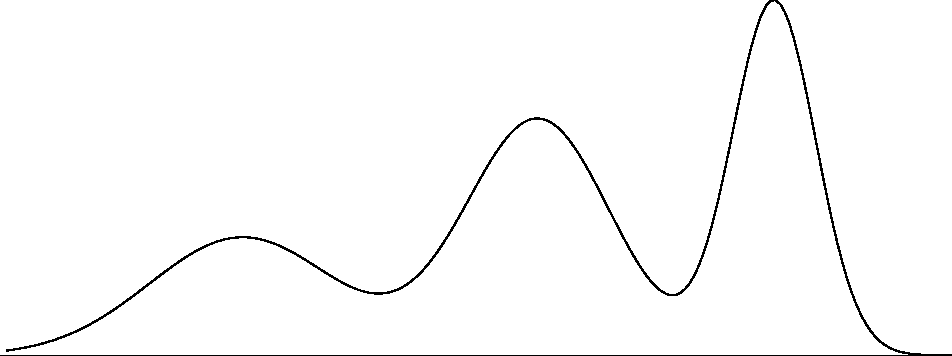
\includegraphics[width=0.4\linewidth]{fig/fig26.pdf}   
\end{figure}

Это обратная задача рассеяния. Качественные рассуждения: введем величину (из \eqref{eq:40}) $\sigma=\frac{\Delta^2 U_m}{12 \beta}=1$. Здесь $U_m$ характеризует нелинейность, а $\beta$ - дисперсию. Предположим, что при $t=0$ задали такое распределение, что $\sigma \ll 1$. Это означает малость $U_m$, мы находимся около стационарного состояния (около нуля). Если мы близки к линейной задаче, главную роль играют дисперсионные механизмы. Есть области прозрачности и непрозрачности. В области прозрачности фазовая скорость у каждой компоненты своя, пакет расплывается.  Приходим к единственному солитону.

Если  $\sigma \gg 1$, преобладает нелинейность. Она порождает новые гармоники. Переход к образованию состава из солитонов. Дисперсия ограничивает частоты, фронт стабилизируется.
